% 导言区
\documentclass{ctexart}

%\usepackage{ctex}       % 中文处理宏包
\usepackage{graphicx}
\graphicspath{{figures/}}   % 图片在当前目录下的figures目录
% 语法:\includegraphics[<选项>]{<文件名>}
% 格式:EPS,PDF,PNG,JPEG,BMP

% 正文区
\begin{document}
    \LaTeX{} 中的插图:

    
\includegraphics[angle=-45, width=0.2\textwidth]{lion.jpg}
    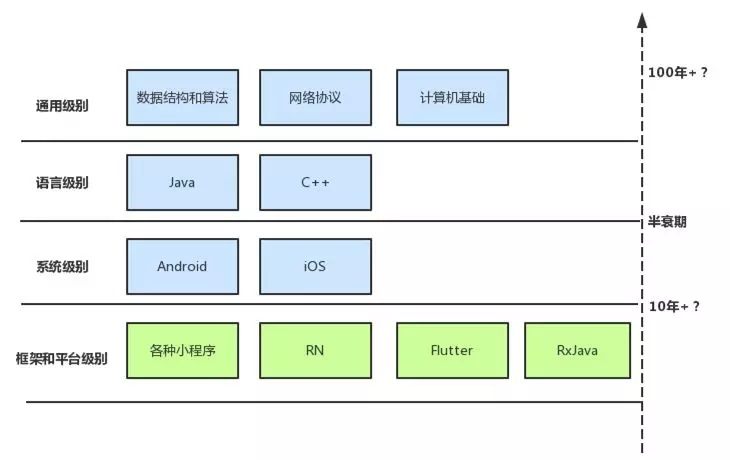
\includegraphics[width=0.2\textwidth]{cs.jpg}
    
\includegraphics[angle=45, width=0.2\textwidth]{conan.jpg}

    
\includegraphics[width=0.2\textwidth]{lion.jpg}
    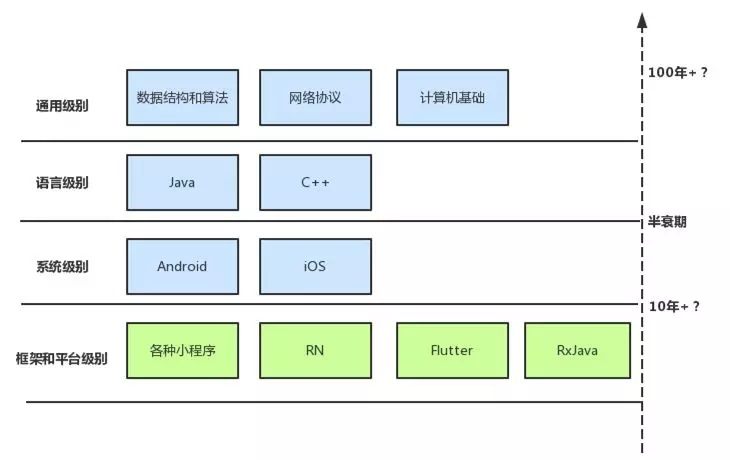
\includegraphics[width=0.2\textwidth]{cs.jpg}
    
\includegraphics[width=0.2\textwidth]{conan.jpg}

    
\includegraphics[height=0.1\textheight]{lion.jpg}
    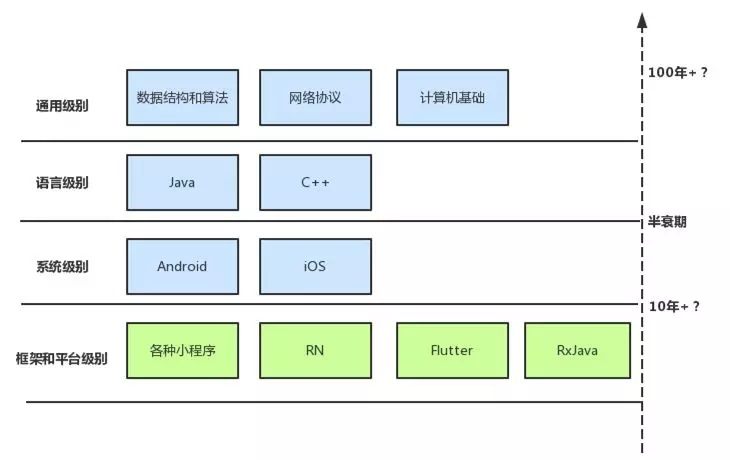
\includegraphics[height=0.1\textheight]{cs.jpg}
    
\includegraphics[height=0.1\textheight]{conan.jpg}

    
\includegraphics[width=3cm]{lion.jpg}
    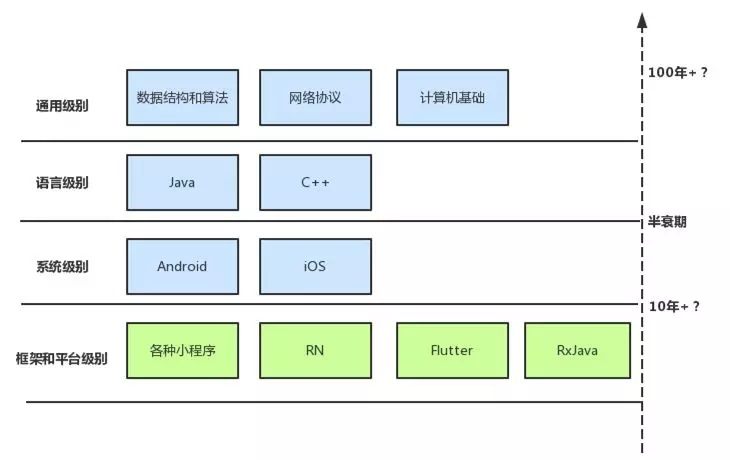
\includegraphics[width=3cm]{cs.jpg}
    
\includegraphics[width=3cm]{conan.jpg}

    
\includegraphics[height=2cm]{lion.jpg}
    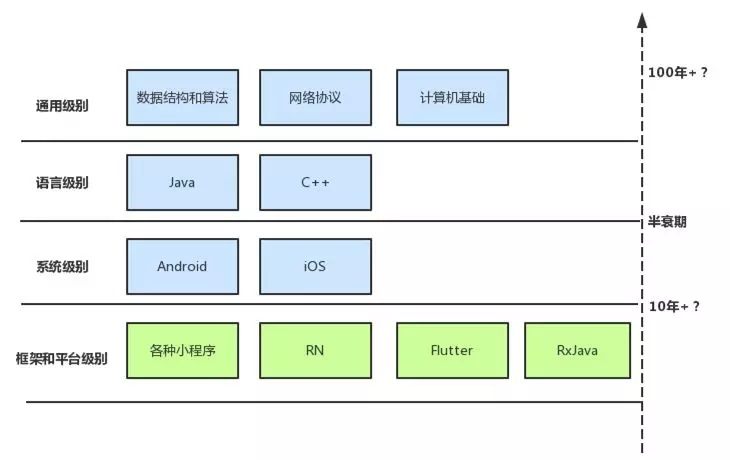
\includegraphics[height=2cm]{cs.jpg}
    
\includegraphics[height=2cm]{conan.jpg}

    
\includegraphics[scale=0.3]{lion.jpg}
    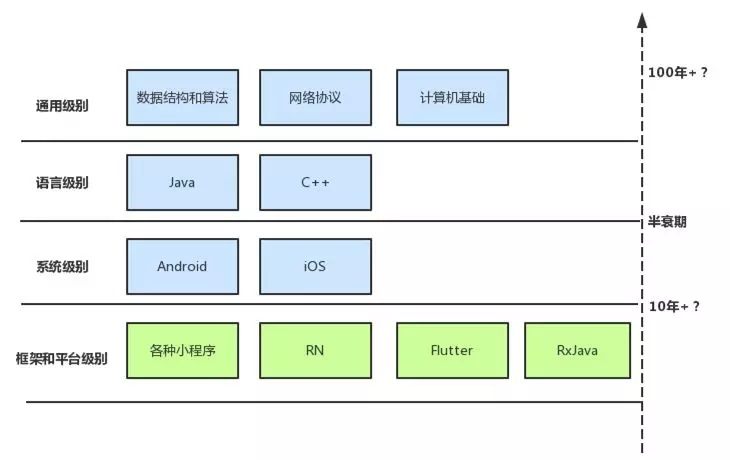
\includegraphics[scale=0.3]{cs.jpg}
    
\includegraphics[scale=0.05]{conan.jpg}

    
\includegraphics{lion.jpg}
    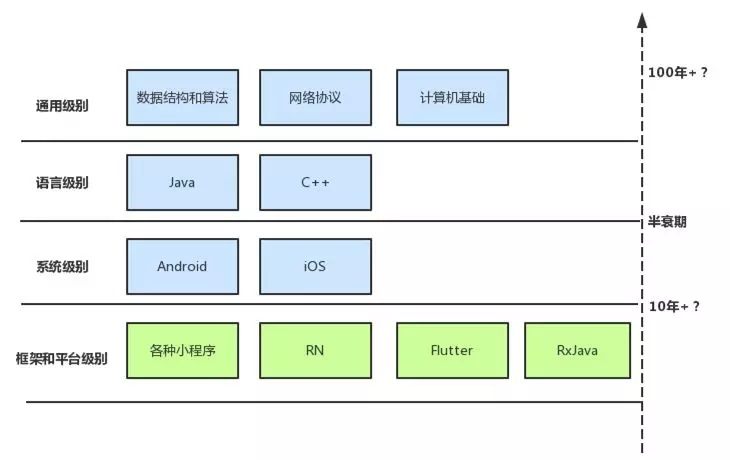
\includegraphics{cs.jpg}
    
\includegraphics{conan.jpg}
   
\end{document}